\documentclass{assignment}
\ProjectInfos{在生活中感知材料的魅力}{GENS1004}{2020-2021学年第一学期}{材料通识课习题}{截止日期 : 2020年11月30日}{陈稼霖}{45875852}
\begin{document}
\noindent\textbf{学生须知:}
\begin{itemize}
    \item[1、] 所有同学须完成全部习题,并均计分;
    \item[2、] 各题分值:【1】-【12】题每题6分,第【13】题20分,第【14】题8分;
    \item[3、] 第【13】题可结合同学本人在课堂上的演讲内容进行叙述,要求图文并茂,禁止从文献或网络大片摘抄;
    \item[4、] 第【14】题为全体同学的必答题,欢迎各位同学提宝贵意见和建议;
    \item[5、] 完成后直接提交到邮箱:zywen@mail.sci.ac.cn;
    \item[6、] 最后提交时间2020年11月30日。
\end{itemize}

\noindent\textbf{题目:}
\begin{ti}
    什么是锂电池和锂离子电池?列举1种典型的锂离子电池体系并描述其原理。
\end{ti}
\begin{da}
    \textbf{锂电池}:广义的锂电池包括锂金属电池和锂离子电池;狭义的锂离子电池特指锂金属电池,即以锂金属单质或锂合金为负极材料的电池,包括\ce{Li/MnO2}电池、\ce{Li/SOCl2}电池等. 由于金属锂是密度最小、氧化还原电位最低的金属,因此锂电池电压高(可达3.9V),比能量高,并且它还有工作温度范围宽($-40\sim 70^{\circ}\mathrm{C}$)、放电平稳、储存时间长的优点。但是锂电池是一种一次性电池,不可循环充电使用,且金属锂非常活泼、容易与电解液发生反应。

    \textbf{锂离子电池}:指的是以锂盐为正极材料的电池。锂离子电池继承了锂电池电压高、比能量高、高低温适应性等优点,最重要的是,锂粒子电池是一种可充电电池。当放电时,\ce{Li+}从负极脱出,经过电介质,在正极得电子转变为锂盐;当充电时,\ce{Li+}从正极脱出,经过电解质嵌入负极。通过这种“摇椅机制”,锂离子电池可以多次充放电使用。

    以\textbf{钴酸锂电池}为例:如图\ref{LiCoO2-battery},其以钴酸锂作为正极,以石墨作为负极,以溶解了锂盐的有机溶剂作为电解质溶液。其工作原理如前所述:当放电时,\ce{Li+}从负极脱出,经过电介质,在正极得电子转变为钴酸锂;当充电时,\ce{Li+}从正极脱出,经过电解质嵌入石墨负极。其反应方程式为
    \begin{center}
        正极:\ce{Li_{1-x}CoO2 + x Li+ + x e- <=>[\text{充电}][\text{放电}] LiCoO2},\\
        负极:\ce{x LiC_6 <=>[\text{充电}][\text{放电}] x Li+ + x e- + x C6},\\
        总反应:\ce{Li_{1-x}CoO2 + x LiC6 <=>[\text{充电}][\text{放电}] LiCoO2 + x C6}.
    \end{center}
    \begin{figure}[H]
        \centering
        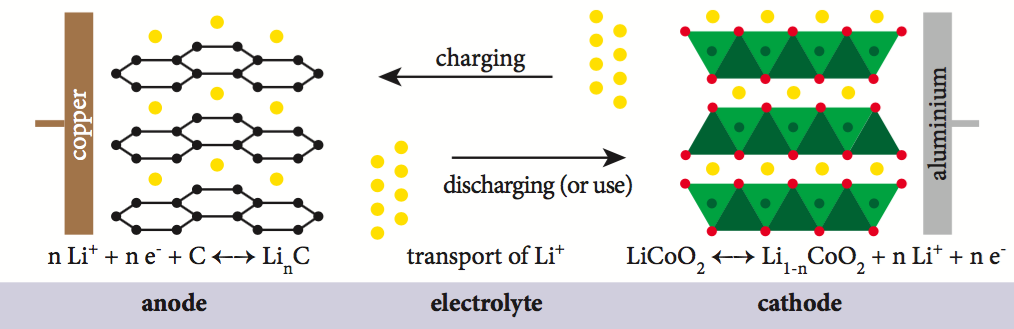
\includegraphics[width=.75\columnwidth]{LiCoO2-battery.png}
        \caption{钴酸锂电池工作原理示意图}
        \label{LiCoO2-battery}
    \end{figure}
\end{da}

\begin{ti}
    有哪些主要的碳材料,石墨烯的主要特点是什么?有哪些主要的应用?
\end{ti}
\begin{da}
    碳材料主要分为四类:
    \begin{itemize}
        \item[(1)] 传统碳材料,如木炭、竹炭、活性炭、炭黑、焦炭、天然石墨等;
        \item[(2)] 特种碳材料,如金刚石、碳纤维、碳分子筛、柔性石墨、氟化石墨;
        \item[(3)] 纳米碳材料,如富勒烯、碳纳米管、纳米金刚石、石墨烯等;
        \item[(4)] 新型碳材料:如课堂上介绍的葡萄藤状的自组装碳纳米管材料、以螃蟹壳为模板的具有扭曲胶合的中空纳米阵列结构的碳材料、火龙果状结构的介孔碳、石榴状结构的空心团簇组成的碳材料、人体肠道绒毛状的碳纤维、碳化的天然木材。
    \end{itemize}

    \noindent石墨烯是一种由单层碳原子以sp$^2$杂化轨道组成六角形蜂窝状结构的二维碳材料,其主要特点有:
    \begin{itemize}
        \item[(1)] 良好的强度和韧性:石墨烯的理论杨氏模量达$1.0$ TPa,固有的拉伸强度为$130$ GPa;
        \item[(2)] 良好的导电性:石墨烯具有sp$^2$杂化形成的大$\pi$键,在常温下的载流子迁移率达$15000\mathrm{cm}^2/(\mathrm{V}\cdot\mathrm{s}$);
        \item[(3)] 良好的导热性:石墨烯的导热系数达$5300\mathrm{W}/\mathrm{mK}$;
        \item[(4)] 良好的吸附能力:作为一种单层二维材料,石墨烯的比表面很大,故可以吸附很多的各种原子和分子;
        \item[(5)] 良好的光学特性:石墨烯在很宽的波长范围内几乎是透明的;
        \item[(6)] 超疏水性和超亲油性:石墨烯在非极性溶剂中表现出良好的溶解性。
    \end{itemize}

    \noindent石墨烯具有广泛的应用,例如:
    \begin{itemize}
        \item[(1)] 电池电极:课堂上提到过,由于石墨烯良好的吸附能力,石墨烯可以用来负载金属锂从而作为锂离子电池的电极;
        \item[(2)] 导电剂:由于石墨烯良好的导电性能,加入石墨烯可以增加介质的导电性能;
        \item[(3)] 单分子气体侦测:由于石墨烯良好的吸附性能以及很大的比表面积,可以通过石墨烯吸附气体分子时的局域电阻变化,侦测气体;
        \item[(4)] 集成电路:作为单层材料,在表面积一定的情况下,石墨烯质量和体积都很小,且具有良好的导电性,故可以用来制作集成电路;
        \item[(5)] 导热材料:石墨烯很薄且导热性很好,适合作为导热材料;
        \item[(6)] 科学研究:石墨烯是一种相对简单的、却又有奇特性质(如上面所述的主要特点,能带中的狄拉克锥以及反常量子霍尔效应等)的二维材料,是材料科学、凝聚态物理研究的热点。
    \end{itemize}
\end{da}

\begin{ti}
    什么是仿生材料学?列举1种仿生材料及其应用。
\end{ti}
\begin{da}
    仿生材料学是指模仿生物的各种特点或特性而研制开发材料的学科,因为在自然选择下,生物的结构往往能进化出具有良好性能和功能的宏观和微观结构,因此仿照生物体结构制备的材料往往也能具有类似的优良属性。

    例如,人们从蜂窝中获得灵感,发明了仿生空心结构材料。蜂窝具有非常良好的结构性能:首先,蜂窝是以正六棱柱的单元紧密排列得到的,这种结构可以以非常少的材料占据非常大的体积,整体的密度很小,其次,蜂窝的结构可以很有效地传导引力,从而具有非常高的强度,最后,蜂窝的多孔结构具有巨大的表面积,从而有较好的吸附能力。

    根据蜂窝的特性,米其林公司设计了一款多孔轮胎\cite{Michelim-porous-tire}(如图\ref{Michelim-porous-tire}),这款轮胎大部分的体积是中空,仅有少部分的骨架结构支撑,因此密度很轻,减少了车辆行驶的能耗,却具有非常高的强度。相比于充气轮胎,这款轮胎日常使用时不需要充气,除了使用过程中造成的磨损之外,不存在被戳破漏气的问题,因此具有较长的使用寿命。此外,在有积水的路面,轮胎的多孔结构可以使得遇到的积水很快地进入和排除轮胎,有效地防止了轮胎的打滑。

    蜂窝是一种牢固又轻巧的建筑,因此人们将类似的结构运用在建筑材料上,发明了蜂窝钢板(\ref{Honeycomb-steel-plate})、蜂窝状混凝土(如图\ref{Honeycomb-concrete})、蜂窝泡沫玻璃(如图\ref{Honeycomb-foam-glass})等建筑材料\cite{Wang2019Application-and-prospect-of-new-bionic-materials}。以蜂窝状混凝土为例,蜂窝状混凝土密度小,常用蜂窝状混凝土的密度等级一般为$300-1200\mathrm{kg}/\mathrm{m}^3$,因此便于运输和安装,且减小了建筑自重。由于蜂窝状混凝土中含有大量封闭的细小孔隙,因此具有良好的保温隔热性能,可以为室内温控节约能源。蜂窝状混凝土还具有较好的隔音性。其中,混凝土是无机材料,不会燃烧,从而具有良好的耐火性,有利于建筑物防火。

    此外,蜂窝状的电极还可用于电池中,既有较好的吸附能力和通透性,便于离子的吸附和传输,还可减轻电池重量。
    \begin{figure}[H]
        \centering
        \subfigure[米其林多孔轮胎]{
            \label{Michelim-porous-tire}
            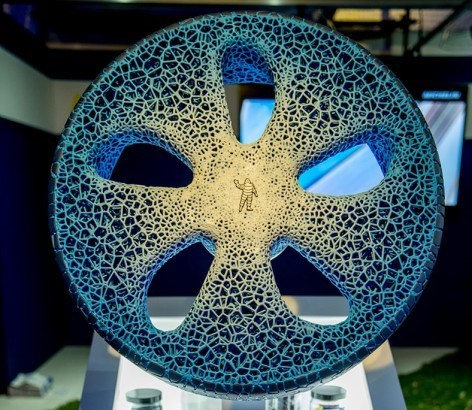
\includegraphics[width=.35\columnwidth]{Michelin-porous-tire.jpg}
        }
        \subfigure[蜂窝钢板]{
            \label{Honeycomb-steel-plate}
            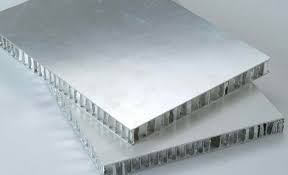
\includegraphics[width=.45\columnwidth]{Honeycomb-steel-plate.jpg}
        }
        \subfigure[蜂窝状混凝土]{
            \label{Honeycomb-concrete}
            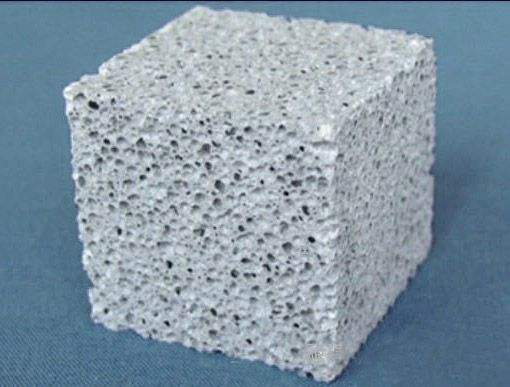
\includegraphics[width=.35\columnwidth]{Honeycomb-concrete.jpg}
        }
        \subfigure[蜂窝泡沫玻璃]{
            \label{Honeycomb-foam-glass}
            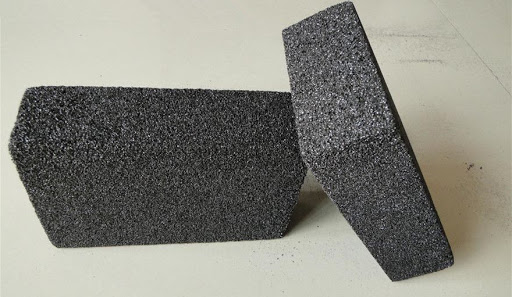
\includegraphics[width=.45\columnwidth]{Honeycomb-foam-glass.jpg}
        }
    \end{figure}
\end{da}

\begin{ti}
    贝壳是一种典型的有机-无机复合材料,具有特殊的结构并赋予其优良的力学性能,请进行具体描述。
\end{ti}
\begin{da}
    贝壳的基本结构大致可分为三部分,最外层为角质层,较薄,主要由硬质蛋白组成,中间为棱柱层,由柱状方解石排列组成,最内层为珍珠母层,是由$95\%$(体积比)的文石碳酸钙和$5\%$(体积比)的柔性生物高聚物(蛋白质和多糖)组成\cite{Zhao2017Preparation-and-application-of-shell-like-mother-of-pearl-layered-composite-material}\cite{Huang2008Research-on-Biomimetic-Composites-with-Shell-Nacre-Structure}\cite{Zhang2006Biomineralization-of-shell-nacre-and-its-enlightenment-to-biomimetic-materials}。

    贝壳珍珠母层的文石碳酸钙晶体片有序沉积所形成的多重微层结构是贝壳优良力学性能的关键来源。珍珠母层的文石碳酸钙晶体片是组成珍珠母层的基本结构单元,多为五、六边形,也存在菱形、混圆形和不规则多边形等多种形态,其宽度一般为$2\sim 20\,\mu$m,厚度约$0.3\sim 0.7\,\mu$m,文石碳酸钙晶体片横向生长使得临近的晶体片相互连接形成微层,微层间以厚约$30$ nm左右的有机基质连接构成珍珠母层\cite{Zhang2006Biomineralization-of-shell-nacre-and-its-enlightenment-to-biomimetic-materials}。这种用有机基质连接无机晶体片形成的微层结构又被称为“砖泥”结构。根据排列方式的不同,贝壳珍珠母层的转你结构可以分为薄板型结构(又称砖墙型结构)和圆柱型结构(堆垛型结构),前者主要存在与双壳类动物(如蛤、扇贝等)的贝壳中,后者主要存在于腹足类动物(如海螺等)的贝壳中\cite{Zhao2017Preparation-and-application-of-shell-like-mother-of-pearl-layered-composite-material}。介观层面上,在薄板型结构中,文石碳酸钙晶体片呈无规则堆叠,横向晶体片的连接处在不同层间相互交错(如图\ref{Shell}(b)(d));在圆柱型结构中,相邻层晶体片的沿垂直层的方向规则排列,其中心位置仅有$20\sim 30$ nm的微小偏移(如图\ref{Shell}(c)(e))\cite{Zhang2006Biomineralization-of-shell-nacre-and-its-enlightenment-to-biomimetic-materials}。微观层面上,文石碳酸钙晶体片表面是粗糙的,其上存在一些宽$10\sim 30$ nm,长$100\sim 200$ nm的凸起以及一些纳米尺度($<10$ nm)的小颗粒,这增强了层与层之间的摩擦作用,防止了层与层之间的滑移,且相邻两层文石碳酸钙晶体片之间被浸没在有机基质中的无机矿物质桥连接在一起,这同样防止了层与层之间的滑移与脱离\cite{Zhao2017Preparation-and-application-of-shell-like-mother-of-pearl-layered-composite-material}。

    \begin{figure}[H]
        \centering
        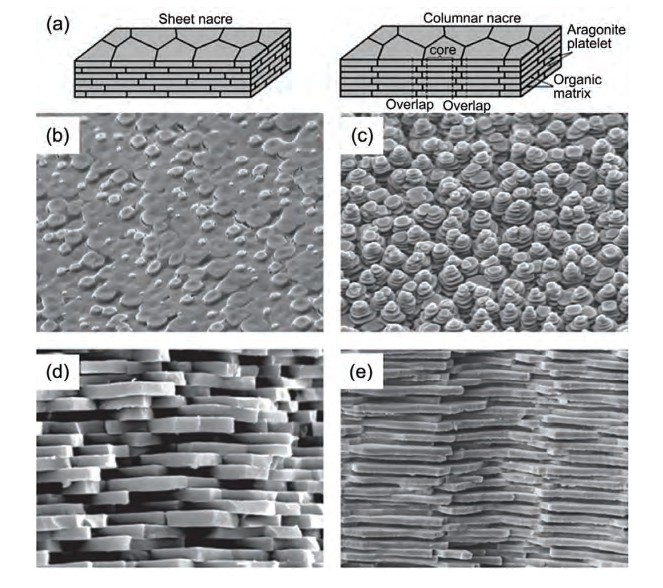
\includegraphics[width=.5\columnwidth]{Shell.jpg}
        \caption{贝壳珍珠母层“砖泥”结构的形貌。(a) 薄板型和圆柱型“砖泥”结构的示意图\cite{wang2012layered};(b)(d)薄板型结构的正面\cite{checa2009key}和截面\cite{barthelat2007mechanics}扫描隧道电子显微镜照片;(c)(e) 圆柱型结构的正面\cite{checa2009key}和截面\cite{rousseau2009dynamics}扫描电子显微镜照片。}
        \label{Shell}
    \end{figure}

    Meyers等人认为,当贝壳受到外界冲击时,无机片层的断裂和相邻无机片层之间的滑动(包括连接相邻无机片层的无机矿物质桥的断裂、无机片层粗糙表面引起的摩擦以及化学键的拉伸等)这两种机制都极大地耗散了外界冲击的能量\cite{meyers2008mechanical}(如图\ref{Shell-2}(c)-(e))。Espinosa等人利用原位原子力显微镜发现脆性的无机片层在纳米尺度会发生一定程度的弯曲,从而使材料的断裂面呈现起伏状,并且会随着片层的滑移而发生界面硬化,这也是一种耗散冲击能量的重要机制\cite{espinosa2011tablet}。此外,裂纹尖端塑性变形\cite{mayer2002rigid}\cite{rabiei2010failure}、裂纹偏转\cite{wang1995observations}\cite{wagner1992relationship}\cite{xia2015nanoasperity}、裂纹钝化\cite{menig2000quasi}、片层拔出\cite{meyers2013structural}(如图\ref{Shell-2}(b))、小尺寸结构单元\cite{gao2003materials}、无机片层表面的阶梯结构\cite{katti2005platelet}、有机基质的变形以及粘附作用\cite{menig2000quasi}和纳米结构的无机片层\cite{jackson1988mechanical}等都对能量的耗散有所贡献。这些能量耗散机制协同作用,造就了贝壳优良的力学性能。
    \begin{figure}[H]
        \centering
        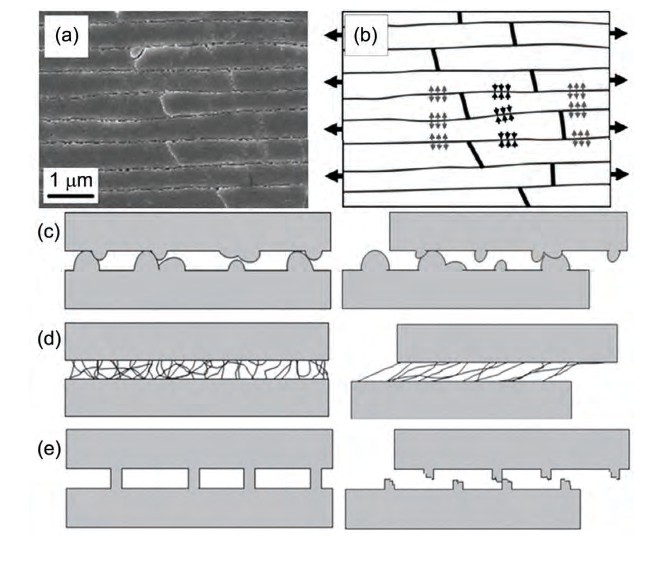
\includegraphics[width=.5\columnwidth]{Shell-2.jpg}
        \caption{贝壳珍珠母层的断裂机制。(a)(b) 微米尺度的断裂形貌和裂纹偏转示意图\cite{barthelat2007experimental};(c)-(e) 纳米尺度无机片层滑动示意图\cite{meyers2008mechanical}。}
        \label{Shell-2}
    \end{figure}
\end{da}

\begin{ti}
    鲨鱼皮有什么结构特征?仿生鲨鱼皮的泳衣是如何实现在水中减阻的?
\end{ti}
\begin{da}
    鲨鱼皮肤并不是一个光滑的表面,而是存在着大量的微小的齿状机构(如图\ref{Shark-skin}),这些微齿结构上含有大量疏水基团的蛋白基体,这些基体可以在鲨鱼皮肤表面形成一层较厚的疏水层\cite{Wang2019Application-and-prospect-of-new-bionic-materials}。

    仿生鲨鱼皮的泳衣使用了仿鲨鱼皮减阻材料,它模仿了鲨鱼皮肤的齿状结构。首先,当水流流过仿鲨鱼皮减阻材料上面的每一个齿状结构,实际上就是流过每一个具有流线型的小结构。齿状的突起顺着水流的方向,具有导流的作用,能够尽量抑制湍流的产生。这样,在游动的过程中,水流能够尽量地贴着泳衣表面,而不会过早脱离而形成湍流,从而避免湍流带来的较大阻力。其次,仿鲨鱼皮材料上的疏水基团的蛋白基体使得材料表面形成一层疏水层,从而降低了水流对材料表面的粘滞阻力。
    \begin{figure}[H]
        \centering
        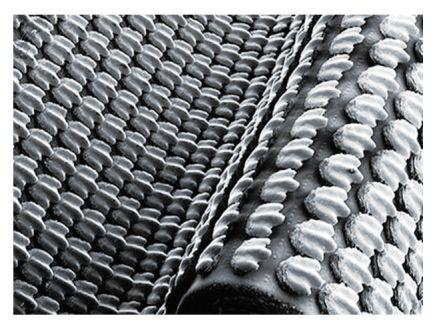
\includegraphics[width=.45\columnwidth]{Shark-skin.jpg}
        \caption{仿鲨鱼皮减阻材料}
        \label{Shark-skin}
    \end{figure}
\end{da}

\begin{ti}
    什么是可再生能源?有哪些典型的可再生能源?可再生能源的主要特点是什么?
\end{ti}
\begin{da}
    \textbf{可再生能源}(Renewable energy)是大自然可以不断自动补充、再生,在人类有生之年都无法耗尽的能源。可再生能源往往直接或间接来自于太阳能和地热能。

    \noindent\textbf{典型的可再生能源}:
    \begin{itemize}
        \item[(1)] 太阳能:直接利用太阳能电池将太阳辐射转化为电能(或者化学能);
        \item[(2)] 风能:太阳照射地球时,各地区的吸热和升温存在不均衡,从而产生气压差,空气流动形成风,用风力驱动涡轮转动发电;
        \item[(3)] 水能/潮汐能:利用水从地势高处向地势低处的流动的、洋流的流动或者潮汐来驱动涡轮转动发电;
        \item[(4)] 生物质能:利用植物或者动物身上的有机物制造的燃料提供的能源(煤炭、石油等化石燃料除外),如生物发酵得到的沼气、燃料乙醇等;
        \item[(5)] 地热能:抽取地壳中的热能作为能量,如用地壳的热量蒸发水成为水蒸气带动涡轮旋转发电。
    \end{itemize}

    \noindent\textbf{可再生能源的主要特点}:
    \begin{itemize}
        \item[(1)] 可再生:如可再生能源的定义,可再生能源可以被大自然不断自动补充、再生,因此取之不尽,用之不竭;
        \item[(2)] 体量大。可再生能源往往直接或间接来自于太阳能和地热能,太阳每秒钟向外发射的能量约为$3.74\times 10^{26}\mathrm{J}$,相当于每秒钟燃烧$1.28\times 10^{16}\mathrm{t}$标准煤所放出的能量。尽管太阳所辐射出来的总能量中只有二十二亿分之一到达地球大气层上界,但其能量也约有$1.73\times 10^{17}\mathrm{W}$,相当于$1.73$亿个百万千瓦级电厂发出的总功率,如果能有效利用这部分能源,那么可再生能源完全可以取代传统化石能源。
        \item[(3)] 环保。不同于传统的化石燃料燃烧会产生二氧化碳以及硫氧化物、氮氧化物,大部分可再生能源(当然生物能源除外)在收集和使用的过程中,基本不会产生二氧化碳和有毒气体,因此对地球的气候、环境更为友好。
    \end{itemize}
\end{da}

\begin{ti}
    硅是地壳中所含的主要元素之一,列举1、2种硅元素的主要应用并加以描述。
\end{ti}
\begin{da}
    \begin{itemize}
        \item[(1)] \textbf{集成电路}:硅是一种半导体,其导电性能可控,就可以充当“开关”的角色,因此以硅为衬底材料的互补金属氧化物半导体(CMOS)是现代微电子集成电路的核心。从沙子中提炼出高纯度硅,通过提拉法长出硅锭,切片成为晶圆,在晶圆上反复刻蚀然后镀上金属层,就可最终制成集成电路,完成复杂的运算。
        \item[(2)] \textbf{光纤}:硅晶体具有较高的折射率,因此光在其中传播时会发生全反射,从而可以将光束缚在硅晶体中传播,这就是硅基波导。晶体硅作为波导的芯层材料具有以下优点:首先,晶体硅具有较高的机械强度和成熟的加工工艺,方便制备高纯度(从而传输损耗小)和大尺寸的晶体硅;其次,晶体硅在通信波段($1.55\,\mu$m)具有较高的透过率和折射率,较高的透过率使得传输损耗较小,而较高的折射率使得波导在做成截面很小的情况下仍然能够良好地束缚传输的光波;最后,在电感耦合等离子体(Inductively coupled plasma, ICP)刻蚀技术的加工下,硅晶体可以形成光滑平整的侧壁,从而有较低的传输损耗,且随着电子束曝光技术(electron beam lithography, EBL)的不断发展,硅基波导的制备精度还在不断提高。
    \end{itemize}
\end{da}

\begin{ti}
    表征材料的亲水结和疏水特性的参数是什么?列举一两种材料的超亲水和超疏水特性应用的实例?
\end{ti}
\begin{da}
    表征材料的亲水和疏水特性的参数是表面接触角,即液体/气体截面接触固体表面而形成的夹角。其中表面接触角又分为表面稳定接触角(即固体表面水平状态下的表面接触角)和表面滚动接触角(即固体表面倾角恰好能使液体在其上滚动状态下的表面接触角)。其中,表面稳定接触角大于$150^{\circ}$且滚动接触角小于$10^{\circ}$的情况被定义为超疏水,表面稳定角小于$5^{\circ}$的情况被定义为超亲水。

    \textbf{超亲水材料的应用}:
    \begin{itemize}
        \item[(1)] \textbf{油水分离}:利用超亲水但超疏水的隔膜分离油状的有机物和水的混合物,可用于物质的提纯和漏油污染的清理;
        \item[(2)] \textbf{物体表面的自清洁}:使用超亲水材料作为物体表面,当用水冲洗物体表面时,水在物体表面并非呈水滴状聚集,而是在物体表面铺展开从而将物体表面与污物分离开,污物顺水流被冲刷走,从而实现物体表面的清洁,可用于玻璃幕墙等建筑物外表面材料。
    \end{itemize}

    \textbf{超疏水材料的应用}:
    \begin{itemize}
        \item[(1)] \textbf{物体表面自清洁}:超疏水材料同样可以实现物体表面的自清洁,使用超疏水材料作为物体表面,则含有污染物的溶液很难吸附在物体表面,且当用水冲洗物体表面时,水珠迅速从物体表面滚落并带走物体表面的污物,从而实现物体表面的清洁,可用于玻璃幕墙等建筑物外表面材料以及防水衣物;
        \item[(2)] \textbf{腐蚀防护}:用超疏水材料对需要防护的物体表面进行镀膜,则即使物体长期处于露天,降水也不会在物体表面长期停留或深入物体内部,从而保持物体干燥,降低物体受腐蚀的速率;
        \item[(3)] \textbf{电子设备防水}:用超疏水材料作为电子设备的外壳,可以防止水进入电子设备的内部,或者用超疏水材料对电子设备内部零件进行镀膜,可以使得电子设备在有水的环境下仍可正常工作,实现电子设备的防水;
        \item[(4)] \textbf{药物缓释}:用超疏水材料作为药品的胶囊或皮衣,可以延缓药物在人体消化系统中的释放时间,并控制药物释放的速率,从而获得更好的药效;
        \item[(5)] \textbf{在锂空气电池中的应用}:锂空气电池在放电的过程中产生的\ce{Li2O2}在潮湿的空气中易转变为\ce{LiOH},\ce{LiOH}难分解,影响电池性能,若能使用超疏水材料作为空气电极,则不易产生\ce{LiOH}。
    \end{itemize}
\end{da}

\begin{ti}
    气垫层是自然界中生物和动物形成超疏水的主要原因,请进行具体描述和说明。
\end{ti}
\begin{da}
    1805年,托马斯·杨最早提出了光滑表面上的接触角公式(图\ref{Contact-angle-microstates}左):
    \begin{align}
        \cos\theta=\frac{\gamma_{\text{SG}}-\gamma_{\text{SL}}}{\gamma_{\text{LG}}},
    \end{align}
    其中$\gamma_{SG}$为固体和气体之间的表面张力,$\gamma_{\text{SL}}$为固体和液体之间的表面张力,$\gamma_{\text{LG}}$为液体和气体之间的表面张力。Wenzel提出,当固体表面存在凹凸状的微结构,且液体与固体表面微结构的凹凸面直接接触(图\ref{Contact-angle-microstates}中),则此时接触角变为$\theta_W$:
    \begin{align}
        \cos\theta_W=r\cos\theta.
    \end{align}
    其中$r$为凹凸面的实际面积与投影面积的比例,它表征了固体表面的粗糙程度。Cassie与Baxter提出,当固体表面存在凹凸状的微结构,且液体仅与固体表面微结构的凸面接触,即液体悬浮在微结构的表面,在液体和固体之间存在气垫(图\ref{Contact-angle-microstates}右),此时接触角变为$\theta_C$
    \begin{align}
        \cos\theta_C=\varphi\cos\theta-(1-\varphi),
    \end{align}
    其中$\varphi$为固体与液体接触面积占当地固体表面凹凸面实际面积的比例。从上述公式中可以看出,在固、液、气材料相同的情况下,当存在气垫,也即Cassie-Baxter状态下,接触角最大,即疏水性最强。
    \begin{figure}[H]
        \centering
        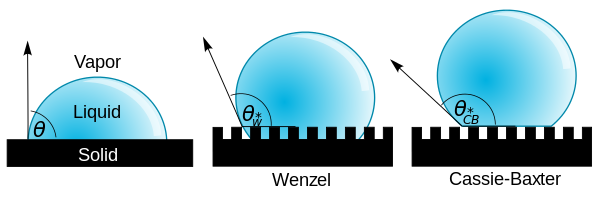
\includegraphics[width=.5\columnwidth]{Contact-angle-microstates.png}
        \caption{各种情况下接触角形成机制的微观结构图。气体环绕的光滑固体表面形成接触角$\theta$;若固体表面存在凹凸状的微结构且液体与固体表面微结构的凹凸面直接接触,则此液滴处于Wenzel状态;若固体表面存在凹凸状的微结构且液体仅与微结构的凸面接触,则此液滴处于Cassie-Baxter状态。}
        \label{Contact-angle-microstates}
    \end{figure}

    各种生物就是通过表面的凹凸状的微结构和液体接触时形成的气垫形成超疏水的。如图\ref{Super-hydrophobic},例如,蝴蝶翅膀表面具有鳞片状的微结构,当水滴落在蝴蝶翅膀上时,会与鳞片间的缝隙之间气垫,因此蝴蝶翅膀表面具有超疏水的特性,使得蝴蝶在雨天仍然可以在空中飞翔;又如,水黾的脚上具有许多密集的油质刚毛,与水接触时形成了很多气垫,这些气垫一方面赋予了水黾的脚以超疏水的性质,另一方面气垫中的空气为水黾提供了额外的浮力,因此水黾可以悬浮在水面上运动而不沉入水底;再如,荷叶表面存在许多微米级的凸起,这些凸起上又有许多纳米级的微粒,当水接触荷叶表面时就可以形成气垫,因此荷叶表面具有超疏水的性质,水珠可以在荷叶表面自由的滚动脱落,减轻了下雨时荷叶支撑的压力。
    \begin{figure}[H]
        \centering
        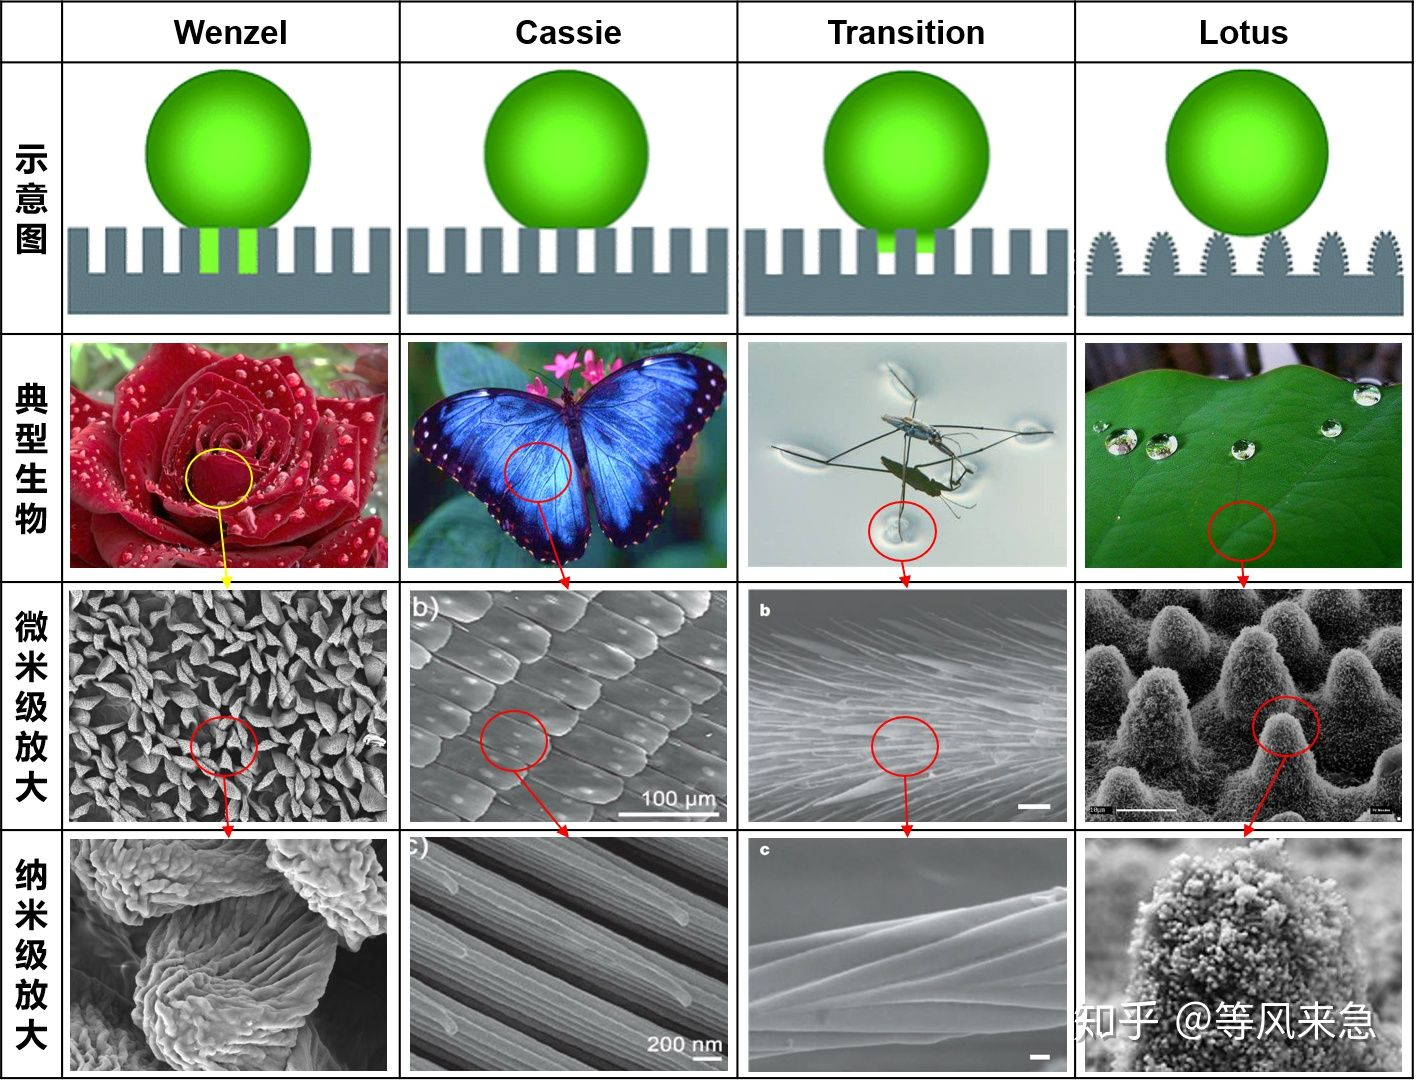
\includegraphics[width=.5\columnwidth]{Super-hydrophobic.jpg}
        \caption{各种生物表面的超疏水结构}
        \label{Super-hydrophobic}
    \end{figure}
\end{da}

\begin{ti}
    柔性可穿戴电子产品有哪些相关技术?列举一种实现柔性电子产品的技术进行描述。
\end{ti}
\begin{da}
    柔性可穿戴电子产品涉及的相关技术包括:
    \begin{itemize}
        \item[(1)] 柔性电子器件;
        \item[(2)] 柔性玻璃;
        \item[(3)] 柔性屏幕;
        \item[(4)] 柔性电池;
        \item[(5)] 柔性电子皮肤;
        \item[(6)] 柔性传感器;
        \item[(7)] 柔性3D打印等。
    \end{itemize}

    以\textbf{柔性电池}为例。与具有固定形状的传统电池不同,柔性电池是一种可以反复弯折而仍然正常工作的电池。通常电池中都包含了正极、负极、隔板、电介质等组件,在柔性电池中,这些组件都要求是柔性的。目前较为常见的做法是将电极材料印刷或黏合在在柔性材料上。目前有报道的包括:用\ce{Li4Ti5O12}和\ce{LiFeO4}作为负极和正极,涂覆在石墨烯上\cite{li2012flexible};或者将负极和正极材料涂覆在碳纳米管上,如基于碳纳米管的钴酸锂电池\cite{hu2010thin}、基于碳纳米管的碳锌电池\cite{hiralal2010nanomaterial}。此外还有将薄膜状有机太阳能电池与超薄锂离子聚合物结合,从而可以在光照下自动充电的柔性锂离子电池\cite{flexible}。由于柔性电池对空间很强的适应性,它可以为柔性可穿戴设备提供电源,或者在某些对空间要求苛刻和需要改变形状的场景下功能,提高电子产品的集成度、小型化程度。
\end{da}

\begin{ti}
    什么是3D打印技术,举例说明3D打印技术的应用。
\end{ti}
\begin{da}
    \textbf{3D打印技术}是一种直接在给定位置叠加相应材料从而制造所需几何形状和材料构成的物件的快速成型技术。在3D打印技术中,首先通过计算机立体建模软件或扫描仪得到包含待制造物件的几何外形和材料构成的数字模型文件,然后将其输入3D打印机,3D打印机根据输入的几何外形和材料构成,控制其喷头的移动和出料,将相应的材料,如金属状粉末、塑料等,堆叠到给定的位置,一层层地构建出所需的物件。3D打印技术具有如下优点:
    \begin{itemize}
        \item[(1)] 由于3D打印技术中直接通过堆叠材料成型,而无需从大块材料切割、钻铣,因此可以减少材料的浪费;
        \item[(2)] 3D打印技术在从设计到打印成型的过程中全程由计算机完成、控制,因此精密度高;
        \item[(3)] 由于3D打印技术全程由计算机控制,且是通过逐层堆叠的方式成型,因此3D打印尤其适合那些形状复杂、具有多层嵌套或空腔结构的物件的制造。
    \end{itemize}

    \textbf{3D打印技术的应用}:
    \begin{itemize}
        \item[(1)] \textbf{传统制造业},如汽车制造业和飞机制造业中,许多零部件具有流线型的结构,工艺复杂,用传统的方法切割会造成较多的浪费,用传统的冲压成型,会导致零件的不均匀,影响其力学性能,而利用3D打印技术一体成型,可以高效而经济地完成这些零件的制造;
        \item[(2)] \textbf{餐饮行业}:餐饮行业中,一些诸如巧克力、糖果、糕点等食物可以利用3D打印技术成型,从而可以设计并实现精巧的外观,给人以美感;
        \item[(3)] \textbf{医疗行业}:除了生产一些无生命的医疗器械外,3D打印还可以生产一些有生命的人体器官,以移植给需要更换器官的病人\cite{kang20163d}。生物学家首先培养出需要的细胞,并且设计好三维数字模型,然后以这些细胞为材料,以数字模型为蓝图,打印出人体器官,打印过程中加入水凝胶以便打印完成后细胞能够粘连在一起形成组织。水凝胶中预留了部分孔洞,有利于血液在组织间流动,有利于组织形成初期的给养和代谢,一段时间后,水凝胶会被无毒地讲解,留出的空腔将发育成血管,最终人造的器官就可以在人体中正常工作;
        \item[(4)] \textbf{新能源领域中的应用}:用3D打印技术可以将碳纳米管、石墨烯等制成具有凹凸结构的石墨电极增大石墨电极的吸附能力,用3D打印技术可以打印石墨电路,从而实现电池部件的精确布局,用3D打印可以制备超薄的电介质陶瓷隔膜,应用与固体氧化物燃料电池中可以提高其效率。
    \end{itemize}
\end{da}

\begin{ti}
    体积变化是很多期间在使用过程中不可避免的问题,请列举一种抑制或缓解材料体积变化的技术措施。
\end{ti}
\begin{da}
    二氧化锡是一种具有极高比容量($782$ mAh/g)的锂离子电池负极材料,但是在锂离子电池工作的过程中,锡电极会由于锂离子的“插入”和“脱嵌”而发生体积的变化。Peng\cite{peng2014synthesis}等人将二氧化锡合成为“苹果状”(如图\ref{Apple-like-SnO2}(a)(c))作为锂离子电池的负极,从而改善了锂离子电池在循环充放电中的性能表现。

    \begin{figure}[H]
        \centering
        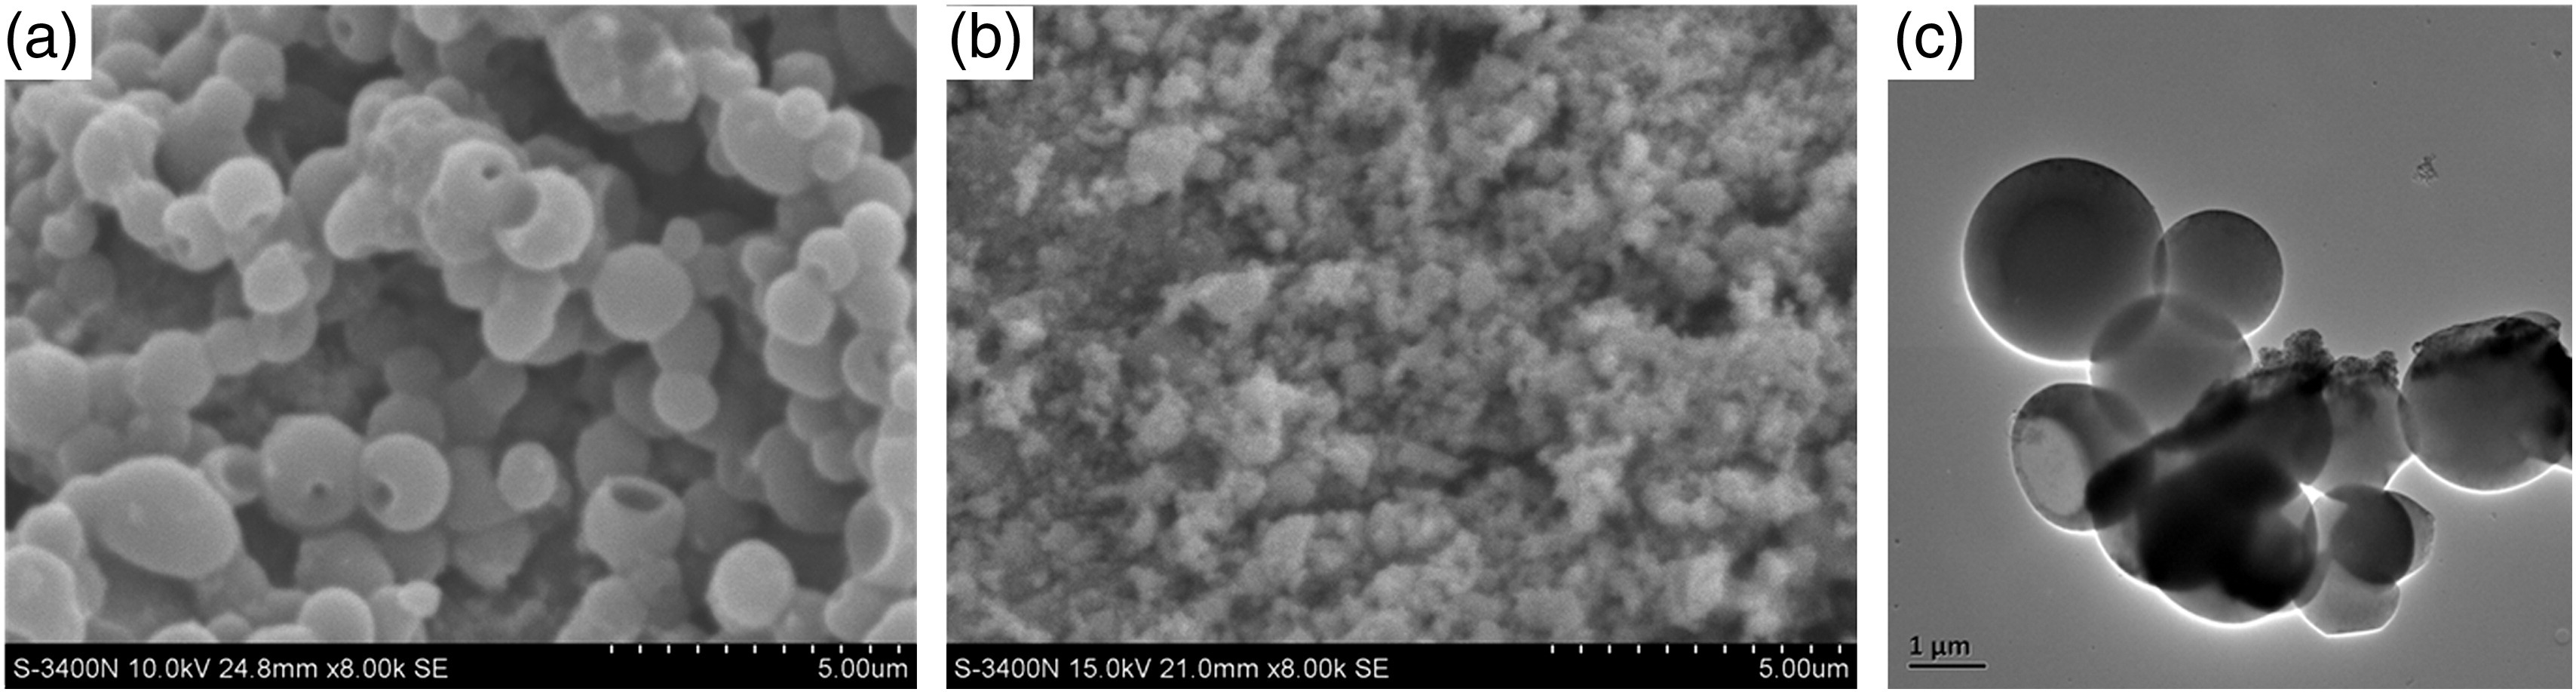
\includegraphics[width=.6\columnwidth]{Apple-like-SnO2.jpg}
        \caption{扫描电子显微镜照片。(a)(c) 苹果状\ce{SnO2}颗粒;(b)普通\ce{SnO2}颗粒}
        \label{Apple-like-SnO2}
    \end{figure}

    如图\ref{Apple-like-SnO2-preparation},首先将用油酸和辛烷作为溶剂,与\ce{Sn4+}离子形成了内部为\ce{Sn4+}离子、外部包裹有机长链的核壳结构,然后在高温下\ce{Sn4+}水解产生\ce{SnO2}微粒。一方面,这些\ce{SnO2}微粒由于较高的表面能,具有聚集的趋势,但同时,外部有机长链的存在导致的位阻效应在一定程度上阻碍了微粒的聚集。在这两种效应的对抗作用下,形成了苹果状的\ce{SnO2}颗粒。
    \begin{figure}[H]
        \centering
        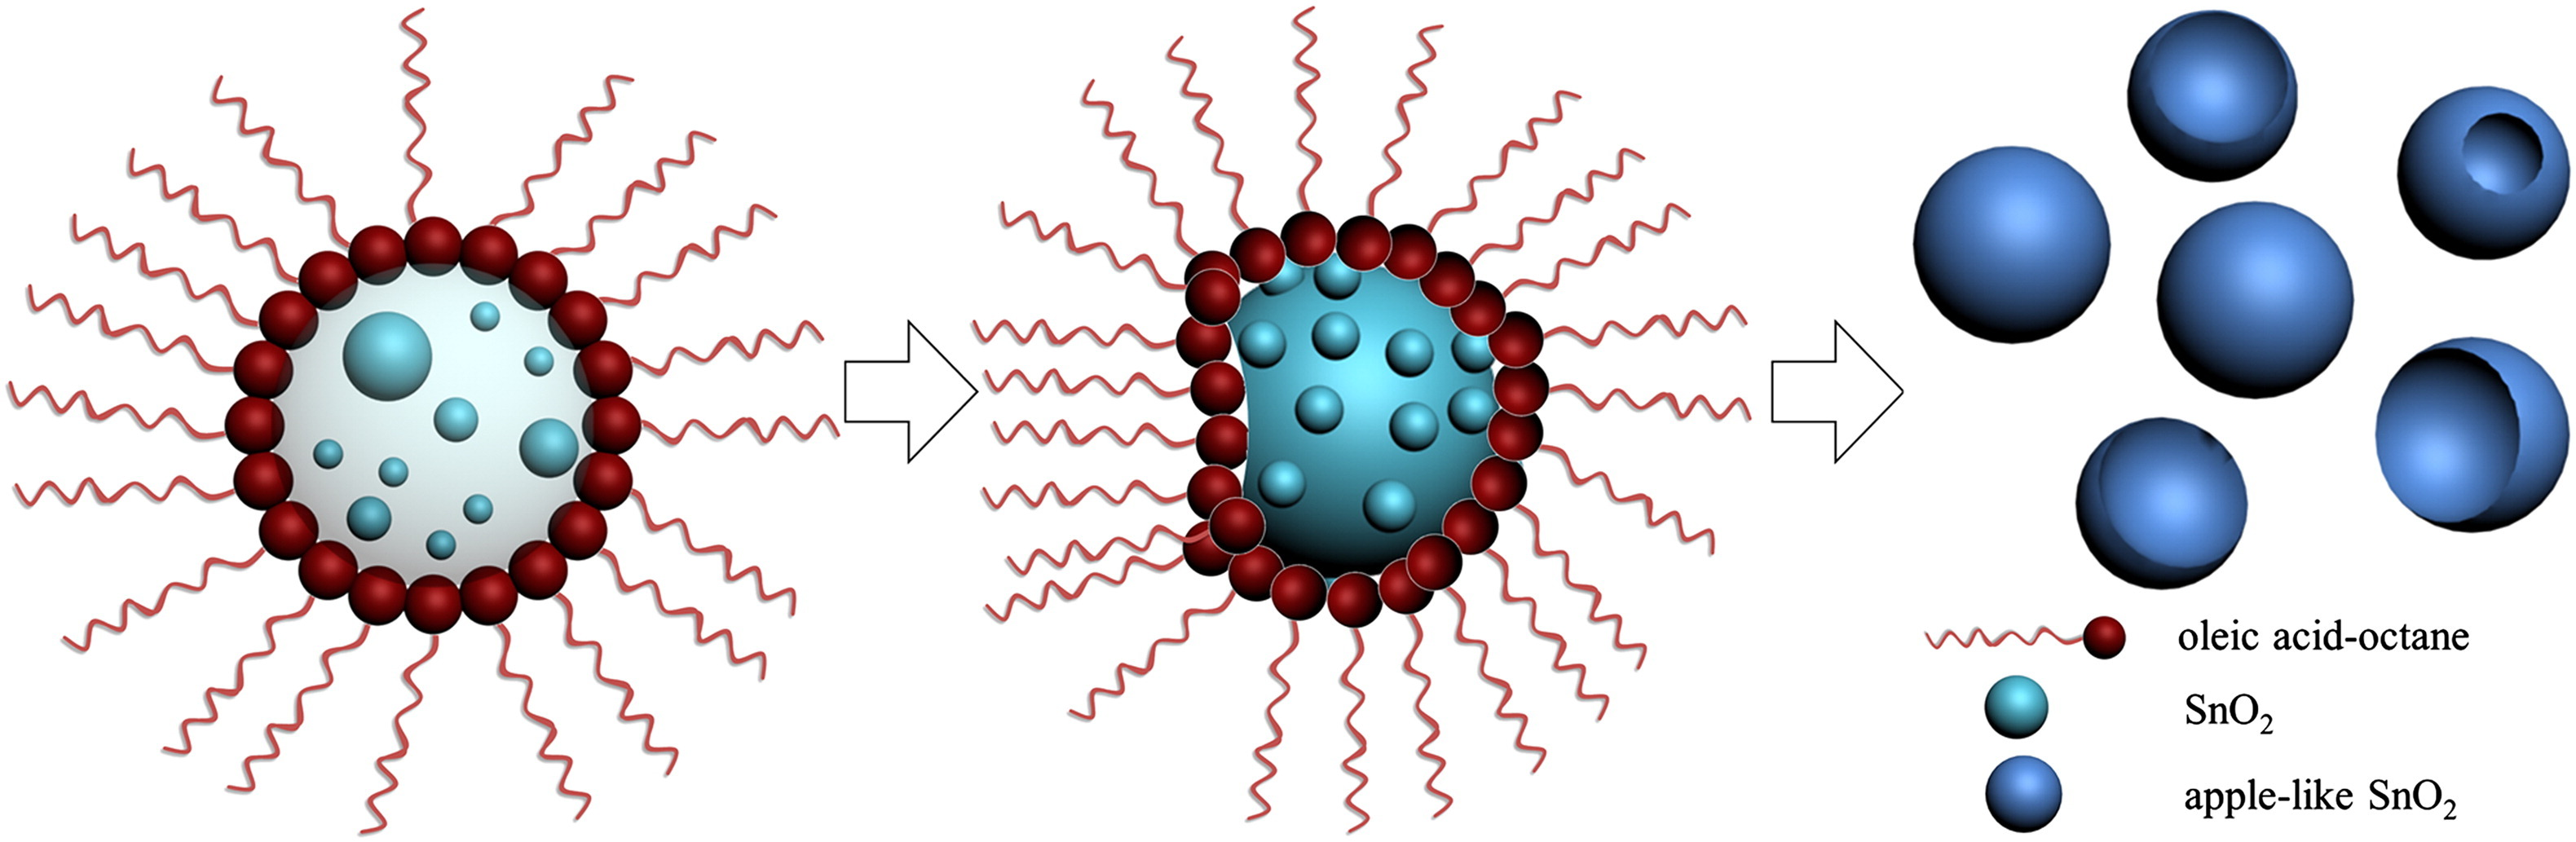
\includegraphics[width=.6\columnwidth]{Apple-like-SnO2-preparation.jpg}
        \caption{苹果状\ce{SnO2}结构的制备过程示意图}
        \label{Apple-like-SnO2-preparation}
    \end{figure}

    在充放电过程中,\ce{SnO2}颗粒将会膨胀,但多出的体积会首先填充苹果状外形的凹陷处,从而避免了颗粒总直径的显著变化,各个颗粒之间不会相互挤压,使得负极保持原有的形状。如图\ref{Apple-like-SnO2-preparation},由苹果状\ce{SnO2}颗粒制成的负极组装的锂离子电池相较普通\ce{SnO2}颗粒制成的负极组装的锂离子电池在充放电循环中比容量损失更缓慢,电压随比容量的变化更加稳定。
    \begin{figure}[H]
        \centering
        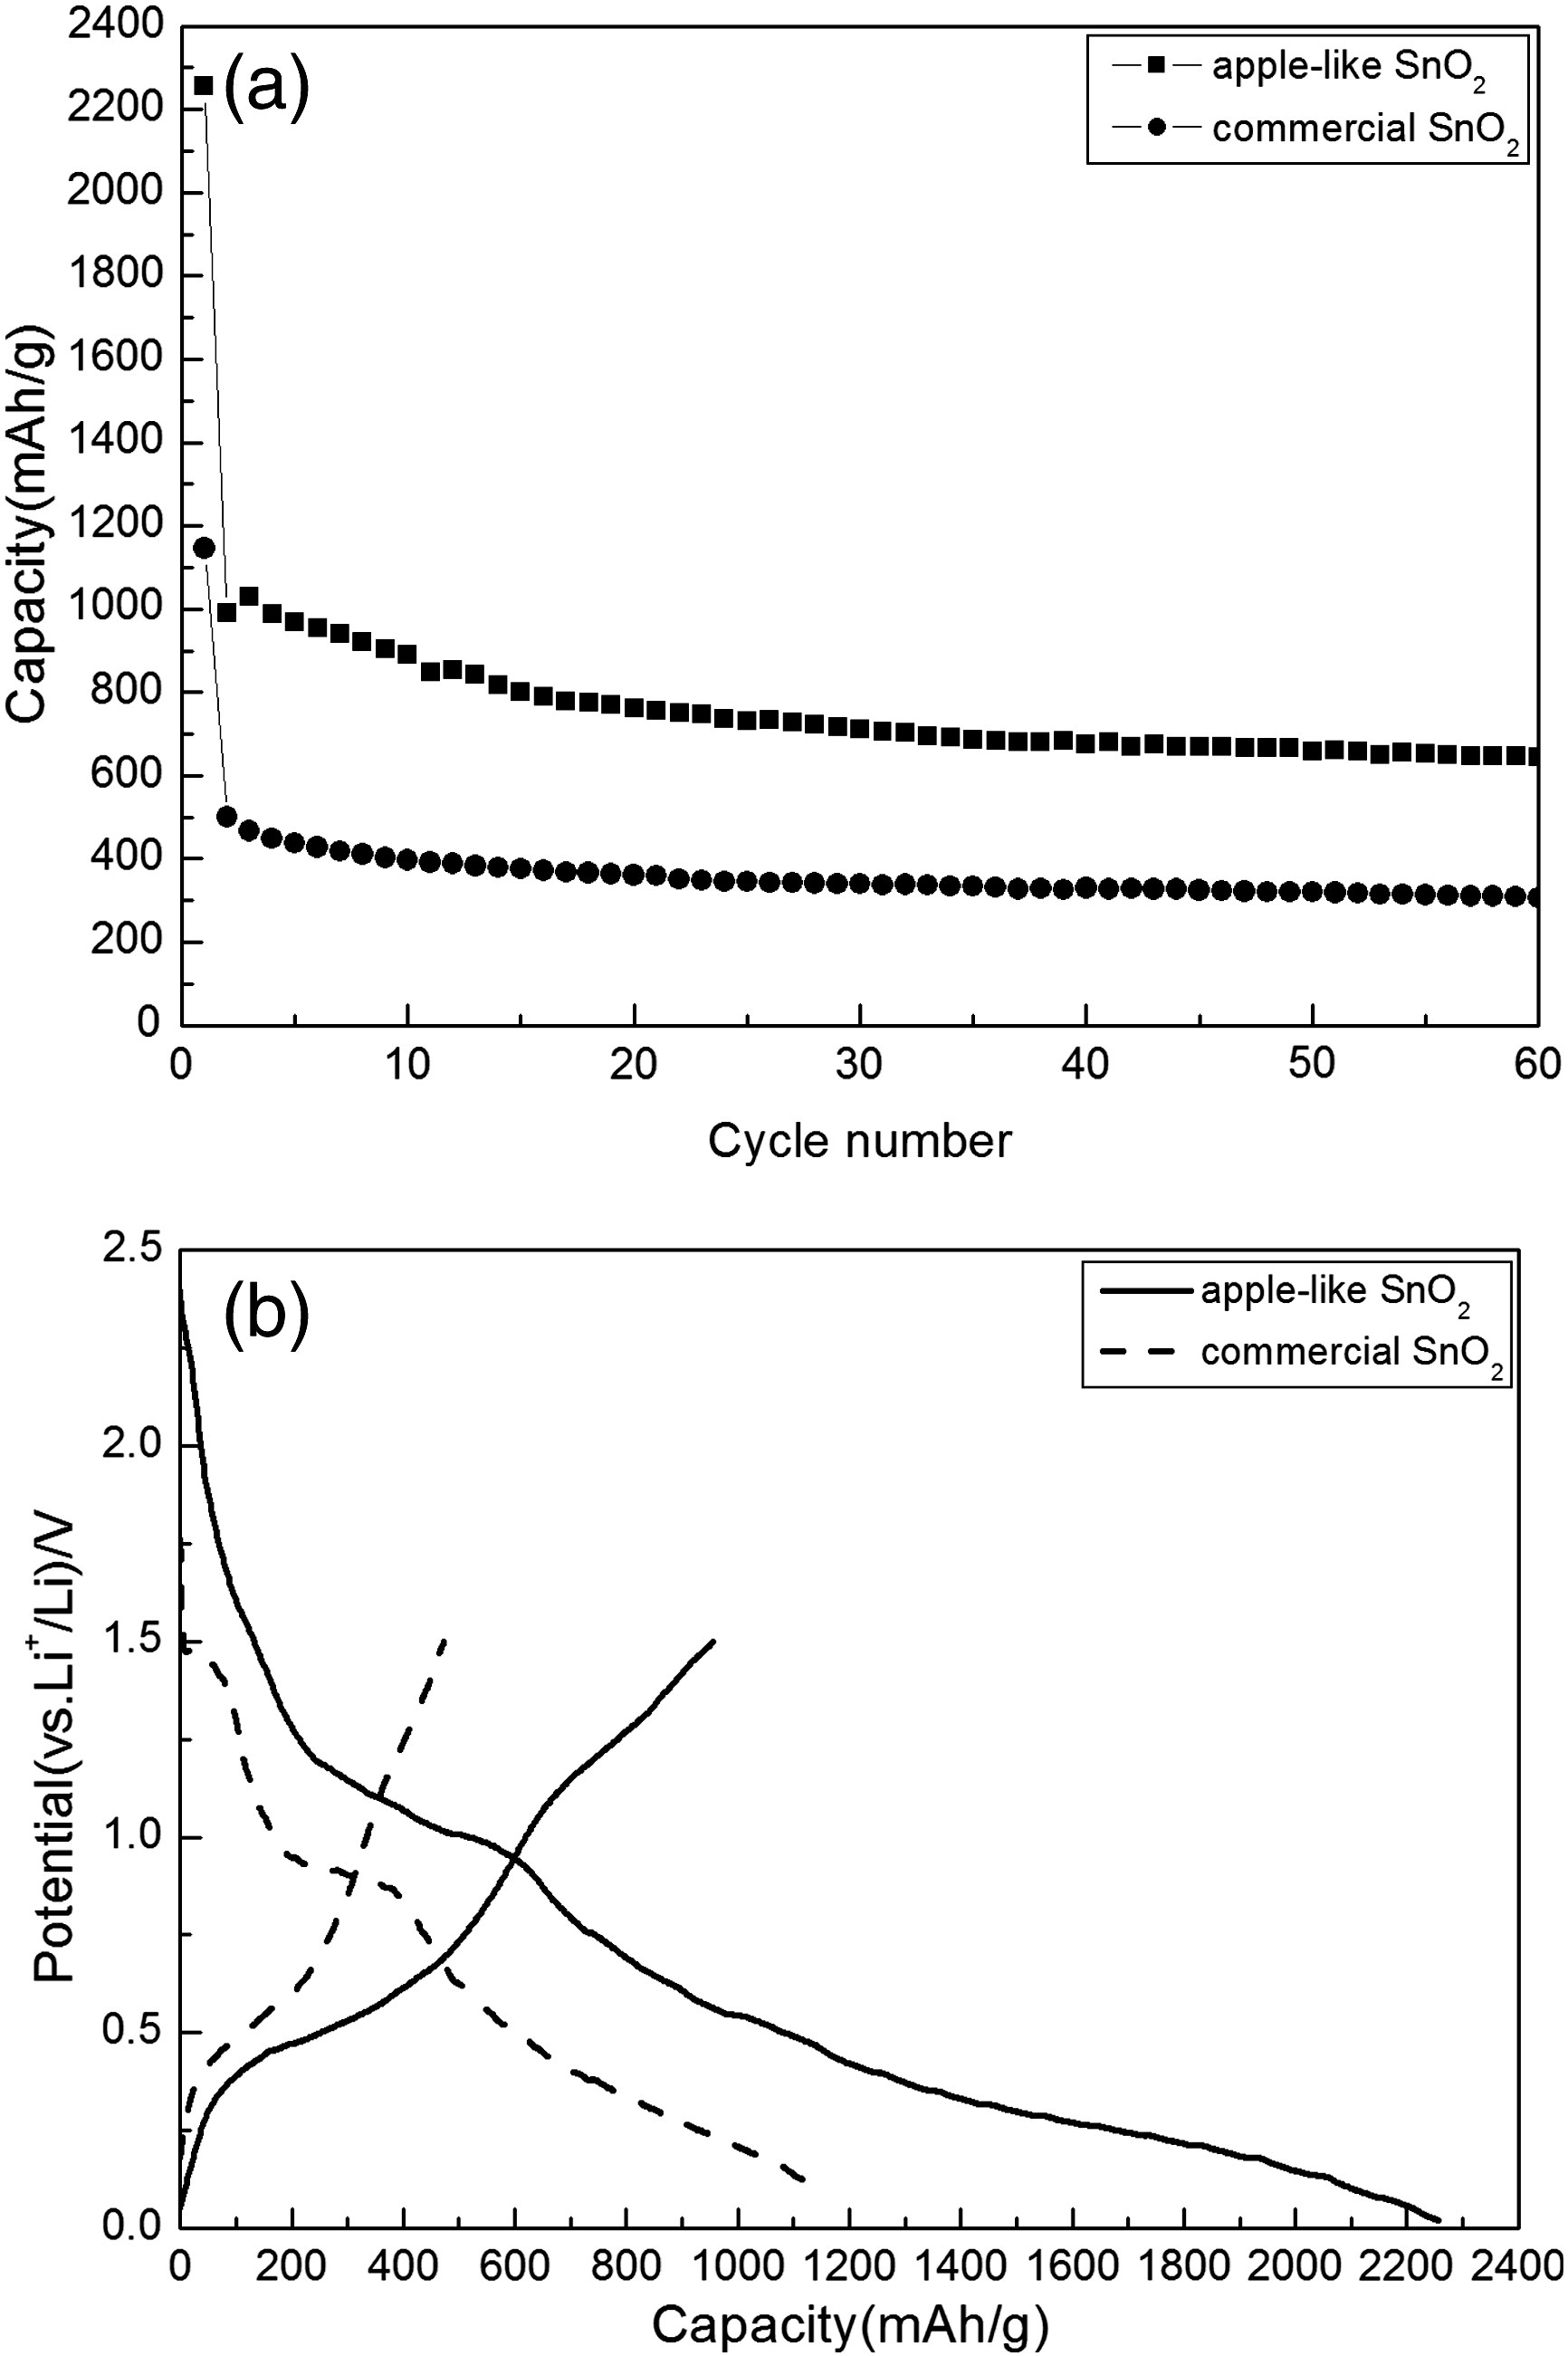
\includegraphics[width=.5\columnwidth]{Apple-like-SnO2-performance.jpg}
        \caption{苹果状\ce{SnO2}负极锂离子电池与普通\ce{SnO2}负极锂离子电池性能测试结果比较}
        \label{Apple-like-SnO2-performance}
    \end{figure}
\end{da}

\begin{ti}
    列举2种由自然界物质引发的新材料技术思维并进行具体描述(不少于1500字)。
\end{ti}
\begin{da}
    \begin{itemize}
        \item[(1)] \textbf{模仿蝴蝶翅膀结构的太阳能电池提高太阳能转化效率。}(参考文献:\cite{siddique2017bioinspired})严重的光损耗制约了传统的薄膜太阳能电池提升其能量转化效率,因此提高对入射光的吸收率有助于改善太阳能电池的能量转化效率。有些蝴蝶,如红珠凤蝶(Pachliopta aristolochiae,如图\ref{Butterfly-Wings})的翅膀即使在明亮的光照下,仍然能够展现出深黑色,也就是说这些蝴蝶的翅膀对光具有很高的吸收率。研究者们从这些蝴蝶的翅膀获得了启发:如果可以制成表面结构与蝴蝶翅膀相近的太阳能薄膜电池,就可以减少太阳能电池的光损耗,进而提高其能量转化效率。

        为此,研究者们仔细研究了红珠凤蝶翅膀黑色区域的结构。他们发现,蝴蝶的翅膀存在很多鳞片状结构,除了鳞片上沉积的黑色色素以外,鳞片上特殊的微纳结构也对光的吸收起到了重要的作用。翅膀的深黑色区域的鳞片上具有径向分布的周期性的微齿,而这些微齿之间又有切向的连接,从而形成了具有无序纳米孔(没有微齿填充的区域就是纳米量级的微孔)的二维网络(图\ref{Butterfly-Wings}(B)(C))。在翅膀内侧的区域,微孔更加密集,黑色也更深,在翅膀外侧的区域,微孔较为稀疏,黑色也较浅(图\ref{Butterfly-Wings}(D))。此外,对于单个鳞片的研究发现,鳞片的凸出部分比鳞片凹陷部分具有更高的吸收率(图\ref{Butterfly-Wings}(E)),这与图\ref{Butterfly-Wings}(D)中的观察相互印证。综上,微孔越密集,鳞片的空气占比越大,吸收率越高
        \begin{figure}[H]
            \centering
            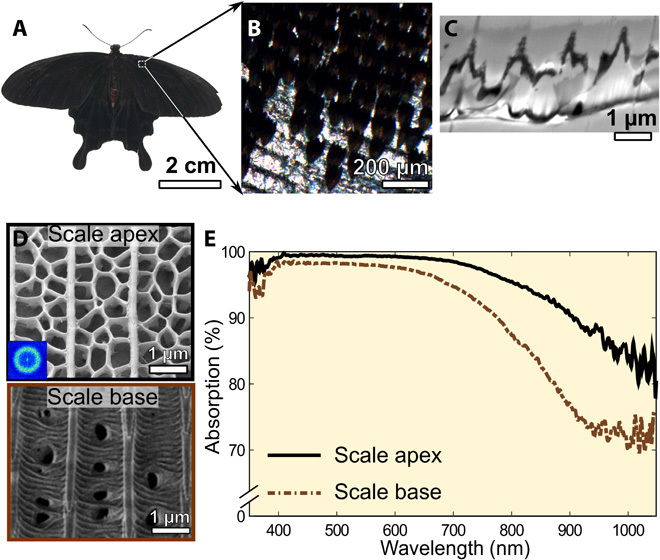
\includegraphics[width=.6\columnwidth]{Butterfly-Wings.jpg}
            \caption{红珠凤蝶的的结构和吸收谱\cite{siddique2017bioinspired}。(A) 红珠凤蝶的照片。(B) 翅膀黑色区域鳞片的微观照片。(C) 黑色区域鳞片截面的扫描电镜图。(D) 鳞片凸起和凹陷部分的扫描电镜图片。(E) 鳞片凸起和凹陷部分的吸收谱。}
            \label{Butterfly-Wings}
        \end{figure}

        为了深入理解这些翅膀上的微纳结构对光学吸收率的影响,研究者还通过有限元分析的方法进一步验证了上面的结论。并且通过有限元分析的方法模拟和优化了材料表面微孔的直径和分布,以得到尽可能高的吸收率。基于此,研究者们按照图\ref{Butterfly-Wings-Fabrication}(A)所示的方法在a-Si:H薄膜上刻蚀出了与蝴蝶鳞片上微纳结构相近的结构,得到了仿生太阳能电池薄膜。从图\ref{Butterfly-Wings-Fabrication}(B)所示的照片中可以感受到这种仿生太阳能电池薄膜相比普通太阳能电池薄膜具有更高的吸收率。
        \begin{figure}[H]
            \centering
            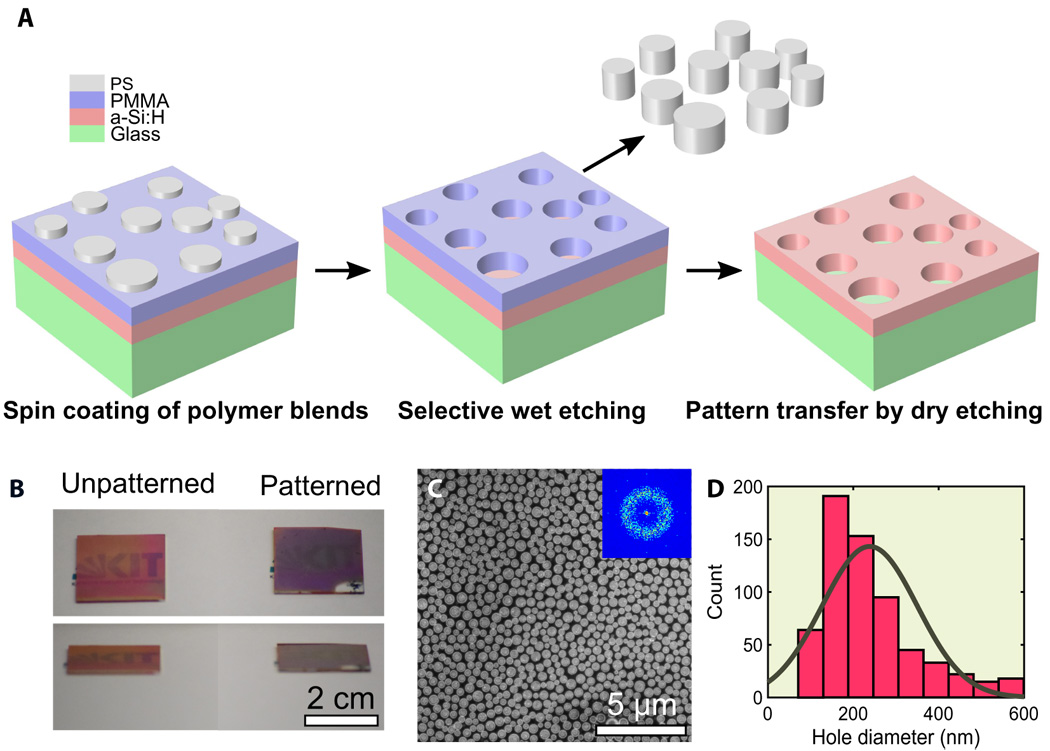
\includegraphics[width=.6\columnwidth]{Butterfly-Wings-Fabrication.jpg}
            \caption{仿生太阳能电池薄膜的制造\cite{siddique2017bioinspired}。(A) 三个主要制造步骤的示意图,首先以玻璃为衬底,在薄a-Si:H层上涂覆聚甲基丙烯酸甲酯(PMMA)和聚苯乙烯(PS)的甲乙酮(MEK)混合溶液,然后选择性显影PS,最后通过干法刻蚀产生a-Si:H层上的图案。(B) 普通太阳能电池薄膜与仿生太阳能电池薄膜的对比。(C) 仿生太阳能电池薄膜的扫描电镜俯视图。(D) 仿生太阳能电池薄膜中微孔直径分布的直方图。}
            \label{Butterfly-Wings-Fabrication}
        \end{figure}

        研究者们对这种太阳能电池薄膜的吸光性能进行了定量的测试。在垂直入射的非偏振光照射下,这种仿生太阳能电池薄膜在各个波段的吸收率均高于普通太阳能电池薄膜(图\ref{Butterfly-Wings-Test}(B))。并且在一定范围内,这种仿生在垂直入射的光照下,这种仿生太阳能电池薄膜的对光的吸收率相比普通太阳能电池的提升百分比随着入射角的增大而增大,例如,垂直入射时仿生太阳能电池薄膜的吸收率相比普通太阳能电池薄膜提高$90\%$,而当入射角为$50^{\circ}$时,这一提升可达$200\%$(图\ref{Butterfly-Wings-Test}(C)),因此这一仿生太阳能电池薄膜特别适用于那些位于中高纬度、太阳高度角较小的区域。
        \begin{figure}[H]
            \centering
            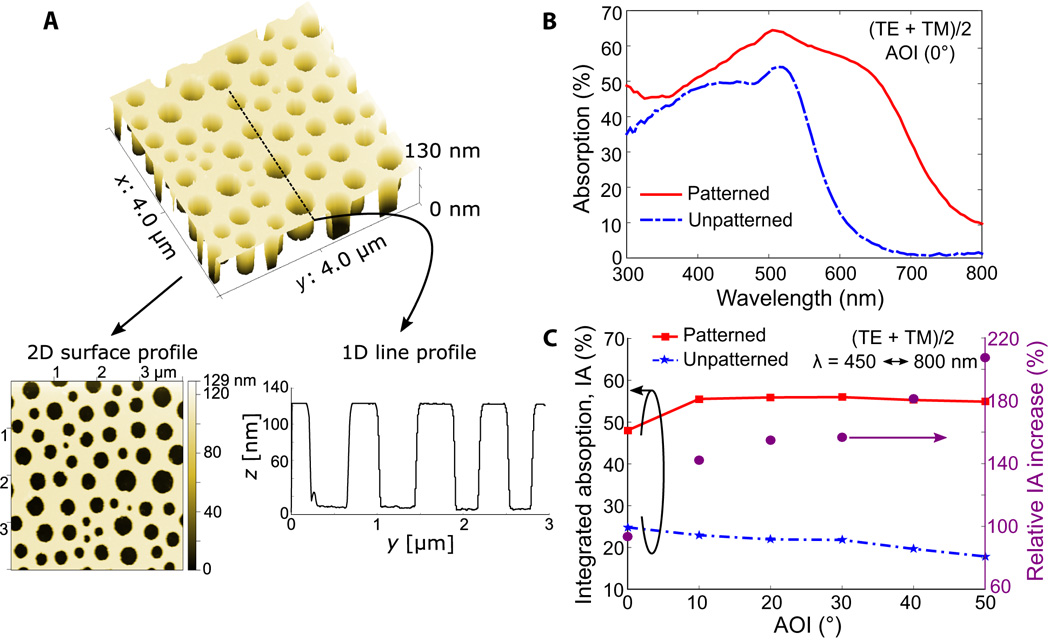
\includegraphics[width=.6\columnwidth]{Butterfly-Wings-Test.jpg}
            \caption{仿生太阳能电池薄膜的表征\cite{siddique2017bioinspired}。(A) 仿生太阳能电池薄膜的3D AFM图像。(B) 仿生太阳能电池薄膜和普通太阳能电池薄膜对垂直入射非偏振光的吸收率对比。(C) 仿生太阳能电池薄膜和普通太阳能电池薄膜吸收率与入射角度的关系。}
            \label{Butterfly-Wings-Test}
        \end{figure}

        \item[(2)] \textbf{源于贻贝的仿生血管黏合凝胶。}(参考文献:\cite{kastrup2012painting})治疗和修补病变或损伤的血管系统是目前医学上的一个难题,因为一般的用药作用于全身而难以在病变和损伤的局部而有效富集,而且缺少可以在体内有血液流动的环境中仍能有效黏合血管的材料。贻贝可以牢固粘连在有水流流动的岩石、码头上,其中的生物黏合方法为研究者提供了灵感。

        研究者们研究了贻贝用于固定自身的黏合剂的组成,发现贻贝与其他物体的黏合处的黏合剂主要由两部分组成,一部分具有较好的生物组织相容性,可以和贻贝自身相结合,另一部分可稳固地吸附在物体上,而这两部分又相互紧密地黏合在一起。模仿这样的结构,研究者们合成了一种仿生黏合凝胶,这种仿生黏合凝胶,包含了藻酸盐(一种具有良好生物稳定性和生物组织相容性的水凝胶)和邻苯二酚(可提供黏合和吸附功能)。

        研究者将这中仿生黏合凝胶用于小鼠的血管壁上,发现这种凝胶在体内环境下可以在较稳定的黏合而不脱落(图\ref{Bio-Adhesive-1}),因此这种凝胶具有用于缝合损伤血管的潜力。此外,这种仿生黏合凝胶可以携带药物并且稳定释放(图\ref{Bio-Adhesive-2}),从而在身体局部形成较高的药物浓度,因此有望用较少的药物精准地治疗癌症等疾病而减轻药物的副作用。
        \begin{figure}[H]
            \centering
            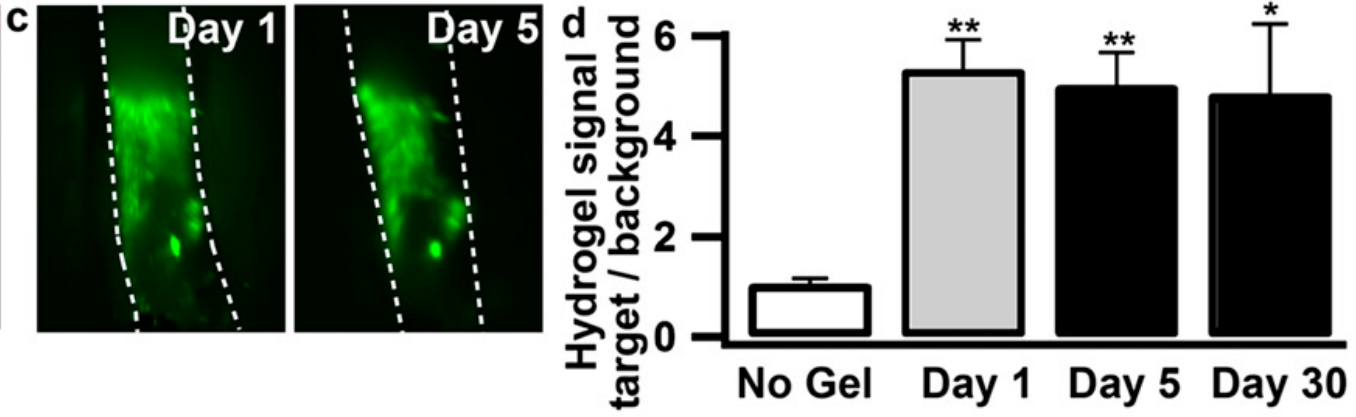
\includegraphics[width=.5\columnwidth]{Bio-Adhesive-1.png}
            \caption{仿生黏合凝胶的吸附性能\cite{kastrup2012painting}。(c) 凝胶植入小鼠体内$1$天和$5$天后的荧光成像。(d) 凝胶植入小鼠后的荧光信号强度随时间变化。}
            \label{Bio-Adhesive-1}
        \end{figure}
        \begin{figure}[H]
            \centering
            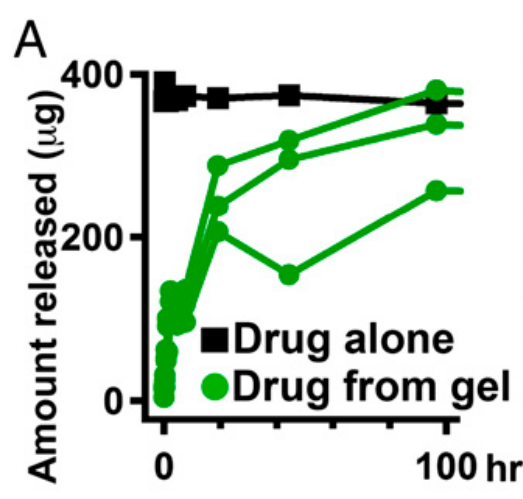
\includegraphics[width=.5\columnwidth]{Bio-Adhesive-2.png}
            \caption{仿生黏合凝胶释放药物量随植入时间的变化\cite{kastrup2012painting}。}
            \label{Bio-Adhesive-2}
        \end{figure}
    \end{itemize}
\end{da}

\begin{ti}
    对本材料通识课的体会、意见和建议。
\end{ti}
\begin{da}
    \textbf{对本材料通识课的体会}:我是物理专业的学生,在我们学院也认识一些材料专业的同学,然而在上这门材料通识课之前,我其实对材料这门学科并不是很了解,甚至有一些不自觉的偏见。我曾误以为材料是新时代的炼金术——我以为材料科学家的工作就是调配各种成分的比例,改变掺杂、制备工艺等各种工程环节,经过大量盲目的实验得到最终想要的材料。

    这门材料通识课证明我是错的。

    首先,我认识到,材料是一门非常科学严谨的学科。它并不是凭空得到灵感,或是通过大量盲目的实验误打误撞、瞎猫碰上死耗子而达到其目的的。材料科学像物理学研究一样,也是需要讲求逻辑、遵循自然的规律的,为了得到并且运用这些规律,材料科学家也和物理学家一样,需要仔细观察自然界中的现象,从这些现象出发展开自己的科研工作。最直接的例子是第二节课所介绍的仿生材料学,例如,材料科学家从贝壳中获得灵感发明了仿生高强度层状符合材料,从蜘蛛丝中获得灵感发明了仿生超强度,从蜂窝中获得灵感发明了仿生空心结构材料,从鲨鱼皮中获得灵感发明了仿生减阻结构材料。

    我发现,材料是一个真正的跨学科的领域。材料的性能和品质不仅取决于其化学组成,也深受其物理结构的影响。例如,超疏水结构不仅来源于材料表面的蜡质成分和憎水基团,还依赖其微米-纳米二级结构。因此材料科学家不仅需要掌握各种制备、检测物质的化学方法,还要理解很多物理知识,借此来指导材料的合成与制备。

    最后,我也惊叹于材料这门学科为人类社会创造的价值。相比物理学家,材料科学家的高明之处在于,物理工作者仅仅尝试对自然界中的现象做出一个解释,他们为人类社会解决各类工程问题、实现各种技术目标提供底层的理论基础,但往往不直接参与解决人类社会的实际问题,因此物理往往对技术的进步常常是间接的、延迟的,而材料学家则并不满足于此,他们在理解了自然界的规律、或是从自然界得到灵感之后,还尝试更进一步地将这些规律运用到材料的制备工程中,在一次次的迭代中不断改进技术、解决问题。材料科学带来了像电池、超疏水的衣物、3D打印技术、柔性可穿戴电子产品这些产品或技术的诞生,它们的影响穿插于人类生产生活的方方面面,并且直接能够直接创造经济效益和改善人类的生活品质。我想这应该是材料这门学科的一大魅力所在。

    \noindent\textbf{意见和建议}:
    \begin{itemize}
        \item[(1)] 在通识课的理论教学中更多地穿插动手实践。去嘉定参观实验室并且动手做实验是一次非常有趣且有意义的教学实践,但是之后的学期,如果选课人数多的话,可能就不是很方便这么做。我们并不一定要去硅酸盐所的实验室,老师也可以联系我们学校的化学或者材料教学实验室,那里的专职的实验教学老师或许能为我们提供教学上的帮助。
        \item[(2)] 希望老师可以在内容的讲解上有侧重。例如,老师上课常常针对某一主题列举很多案例,但是这些例子往往都都是老师阅读过文献后再转述给我们,虽然老师大部分都讲的很清楚,而且也在课件上提供了参考文献,但是内容过的太快,很难给同学们留下深刻印象和理解,大多数同学们课后也很难有动力自己去深入阅读老师上课所讲内容对应的文献。因此,我建议,每节课之前老师都可以布置一到两篇文献的阅读作业,大家在课前针对这一两篇和课堂主题有关的经典文献进行阅读之后,会先对上课的内容有初步的、浅显的理解。然后上课的时候老师对文献所涉及的案例进行重点、具体地讲解(或是请同学们进行讲解,类似组会),也可以和同学们针对文献中的问题进行问答互动,这之后可以对于文献之外的案例可以适当地补充,简略地讲一些其他的例子。我觉得这样的话对于同学们(特别是低年级同学)的文献阅读能力的提高会有很大的帮助。
        \item[(3)] 希望老师可以考虑一下非材料专业或低年级的学生的知识背景。老师上课介绍案例的时候会涉及到一些具体的化学制备、加工方法,一些同学可能并不是很了解,如果方便的话,可以讲解一下具体的原理和过程。
    \end{itemize}
\end{da}

\bibliographystyle{unsrt}
\bibliography{Assignment-Final}
\end{document}